% The twins: Earth twin at x = 0 for 10.6 years; traveller to x = 4.24 ly at
% speed 0.8 and back. Ticks mark each year of each twin's own proper time.
% Traveller: proper time runs at 0.6 of Earth time, so one proper year takes
% 1/0.6 = 1.667 years of Earth time; turnaround at t = 5.3 (tau = 3.18).
\documentclass[tikz,border=1pt]{standalone}
% Shared preamble for the standalone figures: the book's fonts, palette and
% drawing styles. Figures are drawn at their final printed size. A column is
% 3.35in (241pt) wide; a figure across both columns is 7in (505pt) wide.

\usepackage[T1]{fontenc}
\usepackage{newpxtext}
\usepackage[varbb]{newpxmath}
\usepackage[semibold,scale=0.95,lining]{sourcesanspro}
\usepackage{xcolor}
% Palette shared by the book and by the standalone figures in figures/src.
% One main hue (blue), one accent (orange), and a few roles used sparingly.

\definecolor{seblue}{HTML}{1D5B8F}    % headings, worked examples, main curves
\definecolor{seblueDark}{HTML}{123E63}
\definecolor{seorange}{HTML}{DC7A26}  % thought experiments, light and light cones
\definecolor{seteal}{HTML}{1F8577}    % checks, travellers and ships
\definecolor{sered}{HTML}{C0392B}     % negative energy, tension, violations
\definecolor{seviolet}{HTML}{5E548E}  % going deeper
\definecolor{sesand}{HTML}{8C6A3F}    % history
\definecolor{segray}{HTML}{6B7480}    % axes, guides, secondary labels
\definecolor{selight}{HTML}{D5DAE1}   % grids and faint rules

\usepackage{siunitx}
\usepackage{fontawesome5}
\usepackage{tikz}
\usetikzlibrary{arrows.meta,calc,positioning,decorations.pathreplacing,
  decorations.markings,shapes.geometric,fadings,shadings,patterns,3d,
  intersections,backgrounds}
\usepackage{pgfplots}
\pgfplotsset{compat=1.18}
\usepgfplotslibrary{fillbetween,groupplots,colormaps}

\tikzset{
  >={Latex[length=2.1mm,width=1.4mm]},
  every picture/.style={line cap=round, line join=round},
  lbl/.style={font=\sffamily\footnotesize, text=black!85},
  smalllbl/.style={font=\sffamily\scriptsize, text=black!75},
  guide/.style={segray, line width=0.4pt},
  axisline/.style={segray, line width=0.5pt, -{Latex[length=1.7mm,width=1.1mm]}},
  light/.style={seorange, line width=0.9pt},
  lightdash/.style={seorange, line width=0.9pt, dash pattern=on 3pt off 2pt},
  ship/.style={seteal, line width=1.4pt},
  cone/.style={fill=seorange!22, draw=seorange!85!black, line width=0.35pt},
}

\pgfplotsset{
  se axis/.style={
    axis lines=left,
    axis line style={segray, line width=0.5pt, -{Latex[length=1.6mm,width=1.1mm]}},
    tick style={segray, line width=0.4pt},
    major tick length=2.5pt,
    tick label style={font=\sffamily\scriptsize, text=black!75},
    label style={font=\sffamily\footnotesize, text=black!85},
    every axis plot/.append style={line width=1.1pt},
    legend style={font=\sffamily\scriptsize, draw=none, fill=none},
    scaled ticks=false,
    xticklabel={\sansnum{\tick}}, yticklabel={\sansnum{\tick}},
  },
}

% Numbers in figures are set in the sans-serif text font, with a true minus.
\sisetup{mode=text, reset-text-family=false, reset-text-series=false,
  reset-text-shape=false, drop-zero-decimal, group-minimum-digits=5}
% Tick values arrive as long decimals (1.5000000000); parse them first.
\newcommand{\sansnum}[1]{\begingroup\pgfkeys{/pgf/fpu=false}%
  \pgfmathparse{1*(#1)}\num{\pgfmathresult}\endgroup}

\begin{document}
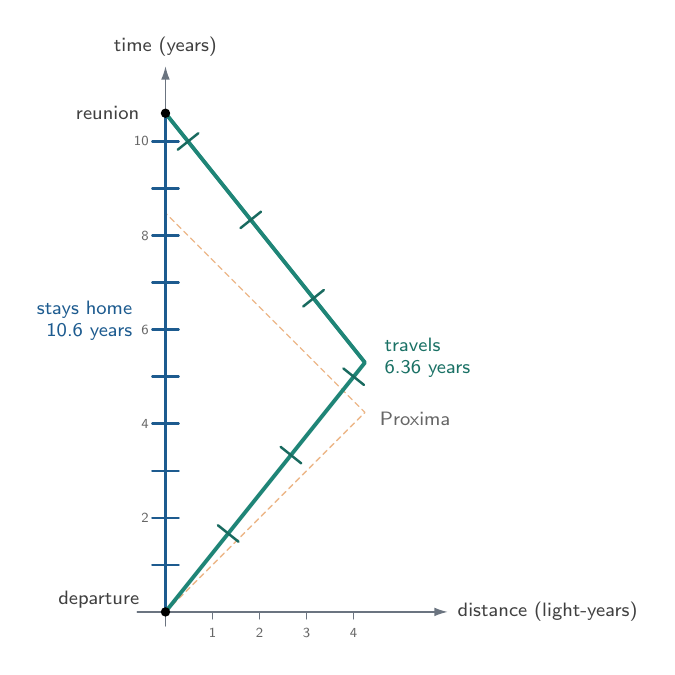
\begin{tikzpicture}[x=17pt, y=17pt]
\draw[axisline] (-0.6,0) -- (6.0,0) node[anchor=west, smalllbl] {distance (light-years)};
\draw[axisline] (0,-0.3) -- (0,11.6) node[anchor=south, smalllbl] {time (years)};
\foreach \x in {1,2,3,4} \draw[segray, line width=0.4pt] (\x,0) -- (\x,-0.15) node[anchor=north, font=\sffamily\tiny, text=black!60] {\x};
\foreach \t in {2,4,6,8,10} \draw[segray, line width=0.4pt] (0,\t) -- (-0.15,\t) node[anchor=east, font=\sffamily\tiny, text=black!60] {\t};
% light to Proxima and back, faint
\draw[seorange!55, line width=0.5pt, dash pattern=on 2pt off 1.5pt] (0,0) -- (4.24,4.24) -- (0,8.48);
% worldlines
\draw[seblue, line width=1.4pt] (0,0) -- (0,10.6);
\draw[seteal, line width=1.4pt] (0,0) -- (4.24,5.3) -- (0,10.6);
% Earth ticks: every year
\foreach \t in {1,...,10} \draw[seblue, line width=0.9pt] (-0.28,\t) -- (0.28,\t);
% traveller ticks: every proper year
\foreach \t/\x in {1.667/1.333, 3.333/2.667, 5.0/4.0}
  \draw[seteal!80!black, line width=0.9pt, shift={(\x,\t)}, rotate=-38.66] (-0.28,0) -- (0.28,0);
\foreach \t/\x in {6.667/3.147, 8.333/1.813, 10.0/0.48}
  \draw[seteal!80!black, line width=0.9pt, shift={(\x,\t)}, rotate=38.66] (-0.28,0) -- (0.28,0);
\fill (0,0) circle (1.7pt);
\fill (0,10.6) circle (1.7pt);
\node[smalllbl, anchor=east] at (-0.35,10.6) {reunion};
\node[smalllbl, anchor=east] at (-0.35,0.25) {departure};
\node[smalllbl, text=seblue, anchor=east, align=right] at (-0.5,6.2) {stays home\\10.6 years};
\node[smalllbl, text=seteal!85!black, anchor=west, align=left] at (4.45,5.4) {travels\\6.36 years};
\node[smalllbl, text=black!60, anchor=west] at (4.35,4.1) {Proxima};
\end{tikzpicture}
\end{document}
